%%%%%%%%%%%%%%%%%%%%%%%%%%%%%%%%%%%%%%%%%%%%%%%%%%%%%%%%%%%%%%%
\subsection{Partitioned Heritability}
%%%%%%%%%%%%%%%%%%%%%%%%%%%%%%%%%%%%%%%%%%%%%%%%%%%%%%%%%%%%%%%

\subsubsection{Flavors of Partitioned Heritability}\label{MV}

Now suppose that instead of estimating total $h^2_g$, we wish to partition heritability into some number of categories;
\emph{e.g.,} functional annotations \cite{gusevregulatory, finucane2014partitioning} or MAF bins \cite{lee2013estimation}.

Formally, let $S$ denote the set of SNPs. 
Suppose we wish to partition $S$ into $p$ non-overlapping annotations $part := {S_1,\ldots,S_p}$ such that 
\begin{equation}
	\bigsqcup_{\alpha=1}^p S_\alpha = S
\end{equation}
and the number of SNPs in category $\alpha$ is $M_\alpha$. Let
\begin{equation}\label{beta}
	\beta := \mathrm{argmax}_\alpha\left( \corr\left[y, \sum_{j\in g} X_j\alpha_j\right]^2 \right).
\end{equation}
Then the partitioned heritability of category $\alpha$ is defined
\begin{equation}
	h^2_S(\alpha) := \sum_{j\in S_\alpha} \beta_j^2.
\end{equation}

Generally one wishes to interpret this quantity as being informative about the biological effect of category 
$C$ on the etiology of $y$.
However, this is not always possible: if the set $g$ is a sparse subset of the set of SNPs that are in LD with SNPs in $g$, then
$h^2_{g,C}$ is contaminated by the effects of non-genotyped SNPs from categories that tend to be in LD with SNPs in $C$.
For example, suppose we have an LD block consisting of ten coding SNPs 
and one intronic SNP in perfect LD, and only the intronic SNP is on our genotyping array. 
In this case, the effects of the ten coding SNPs count towards
$h^2_{g,intron}$, which means that although $h^2_{g,intron}$ tells us about the quality of predictors that we can produce
from genotyped intronic SNPs, it does not tell us about the different biological effects of coding vs intronic SNPs. 
This effect has been observed with real data: 
Gusev et al \cite{gusevregulatory} observed that SNPs in DNAse hypersensitivity sites (DHS)
were enriched for $h^2$ when estimating $h^2$ using a GRM constructed from genotyped and well-imputed SNPs,

We can avoid this problem by making sure that the set of SNPs that we consider is a dense subset of the set of SNPs in LD 
with the set of SNPs that we consider. 
One solution is to use LD information from a sequenced reference panel to estimate partitioned $h^2_{5\myhyphen50\%}$
\cite{buliksullivan2014, buliksullivan2014estimating, finucane2014partitioning} instead of partitioned $h^2_g$.
Continuing the example above, if we estimate LD Scores using sequence data from 1kG \cite{10002012integrated}, 
our LD Scores will take into account the fact that the
genotyped intronic SNP is in LD with ten coding SNPs, and so the $\chi^2$-statistic for the intronic SNP contains more
information about $h^2_{coding}$ than $h^2_{intronic}$.

Another solution is to use both genotyped and well-imputed (\emph{e.g.,} INFO$>$0.9)
SNPs to estimate in-sample LD Scores or construct the GRM.
Note that this requires using a sequenced imputation reference such as 1000 Genomes 
\cite{10002012integrated} or GoNL \cite{genome2014whole}.
Genotyped reference panels such as HapMap 3 \cite{international2010integrating}
are insufficient for partitioning heritability.
This approach will become an increasingly attractive option as the size and quality of available reference panels increase.
The major disadvantage of this approach is that it may be biased if the categories are correlated with imputation quality. 
For example, low MAF SNPs are more difficult to impute that common SNPs, so attempts to partition heritability by MAF 
using imputed data may be confounded by imputation quality.

The magnitude of these problems will vary from partition to partition, and is determined in simulations where phenotypes are generated using a large set of sequenced SNPs, then some of these SNPs are masked before estimating partitioned $h^2_g$.


\subsubsection{Estimators of Partitioned Heritability}

For LD Score regression, instead of using a single vector of LD Scores, we use an $M\times p$ matrix of partitioned
LD Scores \cite{finucane2014partitioning}, where $p$ is the number of categories, and the $\alpha^{th}$ partitioned LD Score
for SNP $j$ is defined
\begin{equation}
	\ell_j^{(\alpha)} := \sum_{k\in S_\alpha} r^2_{jk}.
\end{equation}
We can then estimate partitioned heritability via the multivariate regression equation from \cite{finucane2014partitioning}
\begin{equation}
	\E[\chi^2_j \cond \ell_j ] = 1 + \sum_{\alpha=1}^p \dfrac{Nh^2_S(1)\ell_j^{(1)}}{M_\alpha}  
\end{equation}

For HE regression or REML, we use $p$ GRMs, where the $\alpha^{th}$ GRM is defined
\begin{equation}
	A_{hi}^{(\alpha)} := \sum_{j\in S_\alpha} X_{hj}X_{ij}.
\end{equation}
In this case, the phenotypes are distributed as $y\sim N(0, h^2_S(1)A^{(1)}+\ldots+h^2_S(p)A^{(p)} +(1-h^2_S)I )$,
so the REML estimator is the maximizer of the corresponding likelihood.

The HE regression estimator is defined as follows:
let $B$ denote the $N(N-1)\times p$ matrix
\begin{equation}
B := \left( \begin{array}{ccc}
		A^{(1)}_{hi} & \ldots &  A^{(p)}_{hi} 	\\		
	\end{array} \right)_{h\neq i},
\end{equation}
where rows correspond to pairs of nonidentical individuals and columns correspond to partition elements.
Let $z$ denote the $N(N-1)\times1$ vector $z_{hi} := y_hy_i$.
The HE estimator of partitioned heritability comes from the multivariate regression equation
\begin{equation}
	\E[z_{hi}\cond B] = \sum_{\alpha=1}^p h^2_S(\alpha)A^{(\alpha)}_{hi};
\end{equation}
the closed-form expression for the estimator is
\begin{equation}
	\hat{h}^2_{part,HE} := (\T{B}B)^{-1}\T{B}z.
\end{equation}
Since both the phenotypes $y_i$ and the GRMs have been mean-centered, we do not need to include an intercept term 
(\emph{i.e.,} a column of ones) in $B$.


\subsubsection{Partitioned HE Regression and LD Score Regression}

In the case of partitioned heritability there is still an LD-based interpretation of HE regression, 
but it is not easily interpretable as a modification of one of the standard LD Score regression estimators. 

The numerator of the partitioned HE regression estimator can be rewritten as
\begin{align}
	(\T{B}z)_\alpha 
&=
	\sum_{h<i} A^{(\alpha)}_{hi}y_hy_i\nonumber\\
&=
	\dfrac{1}{M_\alpha} \sum_{j\in S_\alpha} \sum_{h<i} X_{hj}X_{ij}y_hy_i\nonumber\\
&=
	\dfrac{1}{2M_\alpha} \sum_{j\in S_\alpha}\left( \left(\sum_{h} X_{hj}y_h\right)^2 - \sum_h X_{hj}^2y_h^2\right)\nonumber\\
&=
	\dfrac{1}{2M_\alpha N} \sum_{j\in S_\alpha} \left(\chi^2_j - \sum_h X_{hj}^2y_h^2\right)\nonumber\\
&\approx
	\dfrac{1}{2M_\alpha N} \sum_{j\in S_\alpha} \left(\chi^2_j - 1 \right).
\end{align}
The approximation holds in the regime of small effect sizes, by an argument identical to the argument from section 
\ref{HE LD Derivation}.

The denominator of the partitioned HE regression estimator is 
\begin{align}
	(\T{B}B)_{\alpha\beta} 
&= 
	\sum_{h<i}
		 A^{(\alpha)}_{hi}A^{(\beta)}_{hi}\nonumber\\
&= 
	\frac{1}{M_\alpha M_\beta}\sum_{h<i}
		\left(\sum_{j\in S_\alpha} X_{hj}X_{ij} \right)
		\left(\sum_{j\in S_\beta} X_{hj}X_{ij} \right) \nonumber\\
&= 
	\frac{1}{M_\alpha M_\beta}\sum_{h<i}
		\sum_{j\in S_\alpha} 
			\sum_{k\in S_\beta} 
				X_{hj}X_{ij} X_{hk}X_{ik} \nonumber\\
&= 
	\frac{1}{2M_\alpha M_\beta}\sum_{j\in S_\alpha} 
		\sum_{k\in S_\beta} 
			\sum_{h<i}			
				X_{hj}X_{ij} X_{hk}X_{ik}\nonumber \\
&\approx
	\frac{1}{2M_\alpha M_\beta N^2}\sum_{j\in S_\alpha} 
		\sum_{k\in S_\beta} 
			r^2_jk \nonumber\\
&=  
	\frac{1}{2M_\alpha M_\beta N^2} C_{\alpha\beta},
\end{align}
 if we let $C$ denote the $p\times p$ matrix of category-aggregated LD Scores; $C_{\alpha\beta}:= \sum_{j\in S_\alpha}\sum_{k \in S_\alpha} r^2_{jk}$.
The approximation sign is justified by the fact that $\sum_{h<i} X_{hj}X_{ij} X_{hk}X_{ik}$ is an unbiased estimate of $r^2_{jk}/2$.
The $1/N$ upward bias in the usual, biased estimator of $r^2$ comes from the diagonal terms $(X_{ij}X_{ik})^2$.
Let $\mathbf{1}_{part}$ denote an $M\times p$ vector indicating which SNPs belong to which categories.
Then,
\begin{equation}
	h^2_{part,HE} \approx \dfrac{1}{N}C^{-1}\mathbf{1}_{part}(\chi^2-1).
\end{equation}

As usual, REML should be the most efficient estimator of partitioned $h^2_g$ in the multiple VC case,
but it is difficult to draw firm conclusions about the relative efficiencies of HE regression and LD Score regression without
intercept from theory alone, since the efficiency of the default LD Score regression weights will depend on the extent to which the 
categories actually differ.

\subsubsection{Simulations}
 
To simulate a typical use case, I partitioned the same set of chromosome 2 SNPs from section \label{h2:sims}
into ten MAF bins with breakpoints every 5\%.
In these simulations, the genetic architecture was not MAF-dependent, \emph{i.e.,}, none of the bins was enriched for $h^2$ 
relative to the others, and the true value of total $h^2_g$ was 0.5. I performed 1000 simulations in total.
 
The standard errors of the binned estimates are displayed in Figure \ref{Fig:MV},
and the standard errors of the total $h^2_g$ estimates are displayed in Table \ref{Table:mv}.

\begin{figure}[!ht]

\begin{centering}
\caption{Standard Errors of Partitioned Heritability Estimators}
    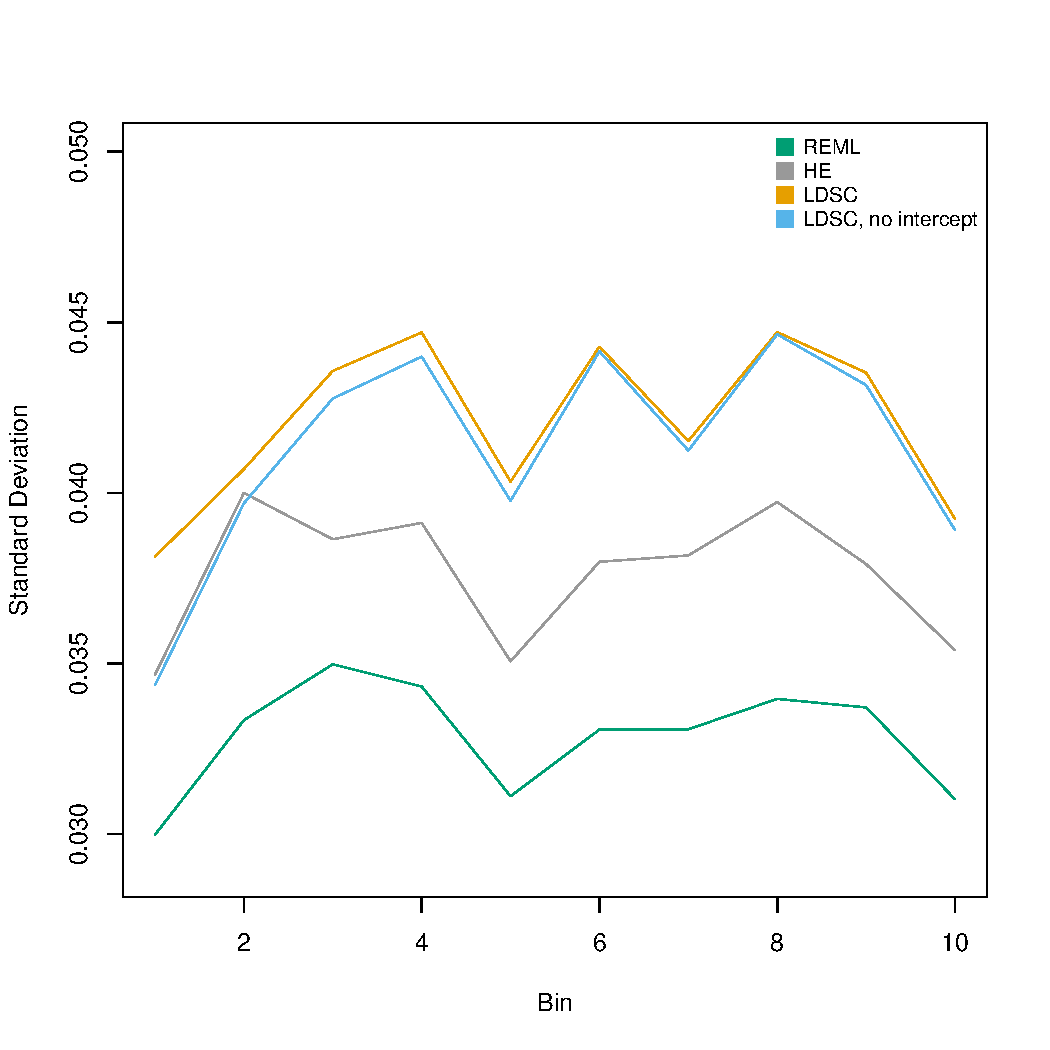
\includegraphics[scale=0.6]{figs/mv.pdf}
         \label{Fig:MV}
         
\small{\textit{This figure displays the standard deviation across 1000 simulations for each of the 10 partitioned $h^2_g$ parameters
from four different estimators.}}
\end{centering}
\end{figure}
\begin{table}[ht]
\centering
\caption{Comparison of Heritability Estimators in Ascertained Samples}
\label{Table:h2hat vs K}
\begin{tabular}{rllll}
\hline
\input{./table/mv}\label{Table:mv}
\end{tabular}

\small{\textit{This table displays the mean and SD of the total $h^2$ estimates from REML, HE regression, and
LD Score regression with and without intercept across 1000 simulation replicates.}}
\end{table}
As usual, REML was more efficient than HE regression or LD Score regression, though 
for partitioned $h^2_g$ estimation from ascertained case/control samples, 
REML will be subject to the same biases as in the single VC case.

The relative efficiency of HE regression vs LD Score regression was less clear in this set of simulations. 
The binned $h^2_g$ estimates from HE regression were more efficient than the binned estimates from
LD Score regression, but the total $h^2_g$ estimates from LD Score regression were more efficient. 
It is not clear whether this is a general trend.
In any event, the differences in SE between HE regression and LD Score regression were not large, and
for partitioned heritability estimation, the distinction between estimating partitioned $h^2_g$ using only genotyped SNPs and 
estimating partitioned $h^2_{5\myhyphen50\%}$ has much more impact on the interpretation of the results
than small differences in SE.

